\documentclass[12pt]{article}
 
\usepackage[margin=1in]{geometry} 
\usepackage{amsmath,amsthm,amssymb}
\usepackage{hyperref}
\usepackage{graphicx}
\usepackage{xcolor}
\usepackage[many]{tcolorbox}
\tcbuselibrary{listings}
\usepackage{listings}

\definecolor{lg}{HTML}{f0f0f0}

\newtcblisting{pycode}{
    colback=lg,
    boxrule=0pt,
    arc=0pt,
    outer arc=0pt,
    top=0pt,
    bottom=0pt,
    colframe=white,
    listing only,
    left=15.5pt,
    enhanced,
    listing options={
        basicstyle=\small\ttfamily,
        keywordstyle=\color{blue},
        language=Python,
        showstringspaces=false,
        tabsize=2,
        numbers=left,
        breaklines=true
    },
    overlay={
        \fill[gray!30]
        ([xshift=-3pt]frame.south west)
        rectangle
        ([xshift=11.5pt]frame.north west);
    }
}

\lstset{
    language=Python,
    basicstyle=\small\ttfamily,
}

 
\begin{document}
 
\title{Exercise 6}
\author{Jari Mattila - 35260T\\
ELEC-E8125 - Reinforcement Learning}

\maketitle

\section*{Task 1}

The training performance plot for Task 1 is presented in Figure~\ref*{fig:fig1} for the continuous Cartpole environment. 
The variance learned as a parameter of the network is applied and TD(0) updates are performed at the end of each episode.
\newline

\noindent
Source files: cartpole\_task1.py, agent.py

\begin{figure}[phb] 
	\centering  % Remember to centre the figure
    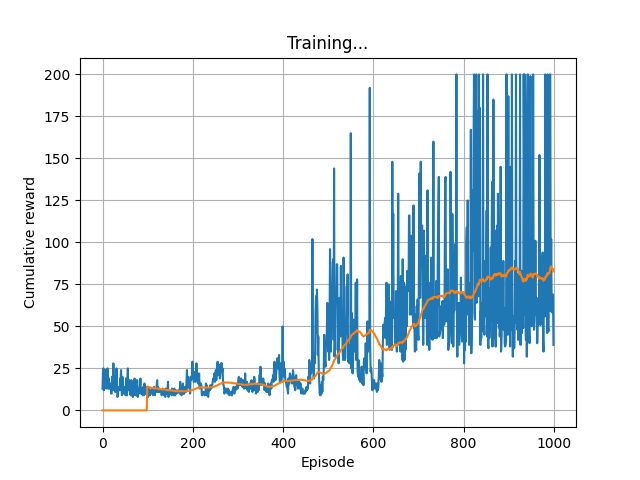
\includegraphics[width=0.9\columnwidth]{img/Figure_1_task_1a_cumulative_reward.png}
	\caption{Training performance using an episodic version of actor-critic algorithm.}
	\label{fig:fig1}
\end{figure}

\pagebreak


\section*{Question 1}

What is the relationship between actor-critic and REINFORCE with baseline?
\newline

In the actor critic algorithm, the baseline in the REINFORCE with baseline method is replaced with the state value function that is updated along episodes by means of least squares over gathered data. 

\section*{Question 2}

How can the value of advantage be intuitively interpreted?
\newline

The value of advantage corresponds to the advantage of choosing a particular action $a$ over the current policy, i.e., how much better is taking action $a$ compared to average (see slide 12 of Lecture 6).


\section*{Task 2}

The training performance plot for Task 2 is presented in Figure~\ref*{fig:fig2}. 
The actor-critic algorithm was updated to perform TD(0) updates every 50 timesteps,
instead of updating the network at the end of each episode. 
\newline

\noindent
Source files: cartpole\_task2.py, agent.py

\begin{figure}[pht] 
	\centering  % Remember to centre the figure
    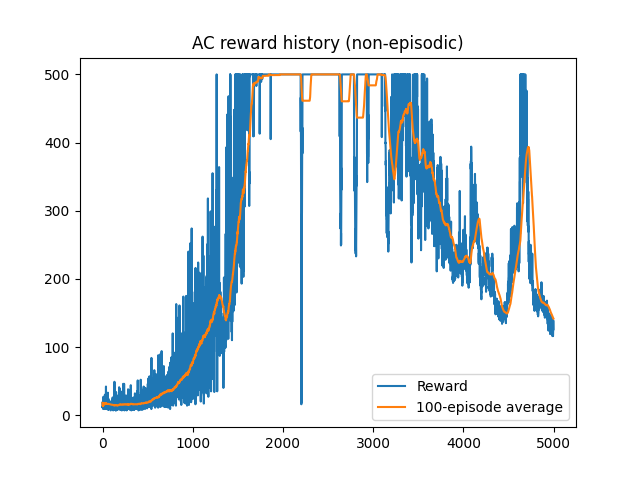
\includegraphics[width=0.8\columnwidth]{img/Figure_2_task_2_cumulative_reward.png}
	\caption{Training performance using a non-episodic version of actor-critic algorithm.}
	\label{fig:fig2}
\end{figure}

\begin{figure}[phb] 
	\centering  % Remember to centre the figure
    \includegraphics[width=0.8\columnwidth]{img/Figure_3_rewards_ContinuousCartPole-v0.png}
	\caption{Training performance using a non-episodic parallel version of actor-critic algorithm.}
	\label{fig:fig3}
\end{figure}


\section*{Task 3}

The training performance plot for Task 3 is presented in Figure~\ref*{fig:fig3}. The actor-critic algorithm was updated to use parallel data collection.
The training was executed using default parameters (8 processes, 8 envs per process) that correspond to 64 parallel environments. 
\newline

\noindent
Source files: parallel\_cartpole.py, agent.py

\pagebreak


\section*{Question 3}

How is parallel data collection different from the parallelism in
multiple\_cartpoles.py script we’ve seen in Exercises 1 and 5? Can it replace multiple runs of
the training algorithm for comparing RL algorithms? \textbf{Explain your answer.}
\newline


Actor Parallel Training
When you use parallel computing with AC agents, each worker generates experiences from its copy of the agent and the environment. After every N steps, the worker computes gradients from the experiences and sends the computed gradients back to the client agent (the agent associated with the MATLAB® process which starts the training). The client agent updates its parameters as follows.
\newline

For asynchronous training, the client agent applies the received gradients without waiting for all workers to send gradients, and sends the updated parameters back to the worker that provided the gradients. Then, the worker continues to generate experiences from its environment using the updated parameters.
\newline

For synchronous training, the client agent waits to receive gradients from all of the workers and updates its parameters using these gradients. The client then sends updated parameters to all the workers at the same time. Then, all workers continue to generate experiences using the updated parameters.


\section*{Question 4}

Figure 1 shows the training performance for all three actor-critic
variants and the REINFORCE algorithm from the last lecture. In terms of initial performance,
REINFORCE seems to completely outperform all tested A2C flavours on Cartpole, despite being
a simpler algorithm. \textbf{Why is it so? Explain your answer.}
\newline

An explanation for the high variance could be because of the returns. For REINFORCE with baseline, I was able to use whitening rewards to normalize the rewards to reduce variance. That was because the algorithm samples the whole trajectory before applying updates, so I was able to apply normalization. 


\section*{Question 5.1}

How do actor-critic methods compare to REINFORCE in terms of
bias and variance of the policy gradient estimation? \textbf{Explain your answer.}
\newline

The actor-critic methods may learn faster than policy gradient because
variance of policy gradient estimate is reduced.


\section*{Question 5.2}

How could the bias-variance tradeoff in actor-critic be controlled?
\newline

Eligibility traces should be used to bring us toward Monte
Carlo methods, but not all the way there. In the future it may be possible to more finely
vary the trade-o↵ between TD and Monte Carlo methods by using variable , but at
present it is not clear how this can be done reliably and usefully (Sutton page 317).

Running with the same data multiple times to avoid bad initialisation.
 

\section*{Question 6}

What are the advantages of policy gradient and actor-critic methods
compared to action-value methods such as Q-learning? \textbf{Explain your answer.}
\newline

Actor-critic approaches allow addressing continuing
problems and continuous action spaces. 
\newline

However, they are actually different internally. The most fundamental differences between the approaches is in how they approach action selection, both whilst learning, and as the output (the learned policy). In Q-learning, the goal is to learn a single deterministic action from a discrete set of actions by finding the maximum value. With policy gradients, and other direct policy searches, the goal is to learn a map from state to action, which can be stochastic, and works in continuous action spaces.
\newline

As a result, policy gradient methods can solve problems that value-based methods cannot:
\newline

Large and continuous action space. However, with value-based methods, this can still be approximated with discretisation - and this is not a bad choice, since the mapping function in policy gradient has to be some kind of approximator in practice.
\newline

Stochastic policies. A value-based method cannot solve an environment where the optimal policy is stochastic requiring specific probabilities, such as Scissor/Paper/Stone. That is because there are no trainable parameters in Q-learning that control probabilities of action, the problem formulation in TD learning assumes that a deterministic agent can be optimal.
\newline




\bibliographystyle{ieeetr}
\bibliography{template}  % Modify template with your bibliography name
\end{document}
